\chapter{Introdução}

Esta aventura leva os novos agentes da ANVESN a Barra das Garças, onde uma série de eventos sobrenaturais ocorre em locais emblemáticos. Inicialmente, a missão envolve uma suposta assombração no cemitério, mas logo revela a presença de um extraterrestre em dificuldades, perseguido por intraterrenos que o veem como uma ameaça. Para resolver o caso, os agentes precisarão interagir com a população local, explorar locais secretos e monitorar atividades estranhas em cavernas subterrâneas.

Barra das Garças, localizada na região Centro-Oeste do Brasil, é conhecida por sua diversidade cultural e pela presença de mitos e lendas que se misturam ao cotidiano dos moradores. Com uma população aproximada de 61 mil habitantes, a cidade é um importante centro turístico graças às suas atrações naturais, como a Serra do Roncador e a confluência dos rios Araguaia e Garças. Barra das Garças também é considerada um ponto místico e esotérico, atraindo curiosos e entusiastas do sobrenatural. A cidade é famosa por lendas de portais para outras dimensões e avistamentos de OVNIs, que contribuem para a atmosfera de mistério que cerca a região.

\begin{figure}
    \centering
    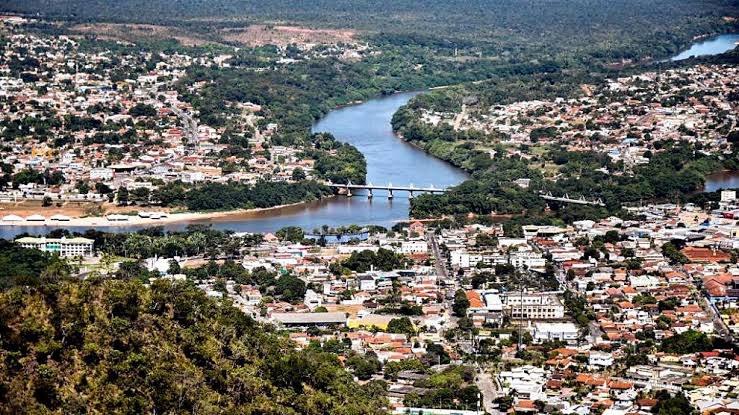
\includegraphics[width=0.8\linewidth]{barra.png}
    \caption{Foto da Cidade}
    \label{fig:cidade}
\end{figure}

Uma das figuras mais emblemáticas da região é o coronel inglês Percy Fawcett, que desapareceu em 1925 durante uma expedição na Serra do Roncador, enquanto buscava uma cidade perdida chamada Z. Esse desaparecimento misterioso inspirou filmes e livros ao redor do mundo, aumentando o fascínio pelas lendas da região. A Serra do Roncador é amplamente conhecida por seus mistérios e atrai inúmeros curiosos que buscam entender mais sobre o local. Existe um ``discoporto'' em Barra das Garças, que seria um suposto aeroporto para discos voadores, construído para facilitar o contato com seres de outros planetas. Segundo os relatos locais, há menções frequentes de avistamentos e aparições de luzes misteriosas que, para muitos, reforçam a crença na presença de vida extraterrestre na região.

A Gruta dos Pezinhos é outro local intrigante, conhecida por suas marcas petrificadas que muitos consideram um exemplo do misticismo local. Margherita de Tomas, jornalista e escritora italiana que estuda o desaparecimento de Fawcett, visitou a gruta e afirmou que os pés com diferentes números de dedos podem ser explicados como casos de polidactilia ou mesmo mutilações, aumentando ainda mais o caráter enigmático do local.

De acordo com a reportagem da BBC, os mistérios da região também envolvem lendas de intraterrenos - seres que vivem em cidades subterrâneas e que estão em constante vigilância para proteger seus domínios de possíveis invasores. Essas histórias, contadas por gerações, reforçam a crença de que há portais e caminhos secretos que levam a mundos escondidos abaixo da superfície. O coronel Percy Fawcett estava em busca desses mistérios quando desapareceu, e muitas das teorias locais apontam que ele poderia ter encontrado uma dessas entradas, levando ao seu desaparecimento.

% \begin{figure}[hbt]
%     \centering
%     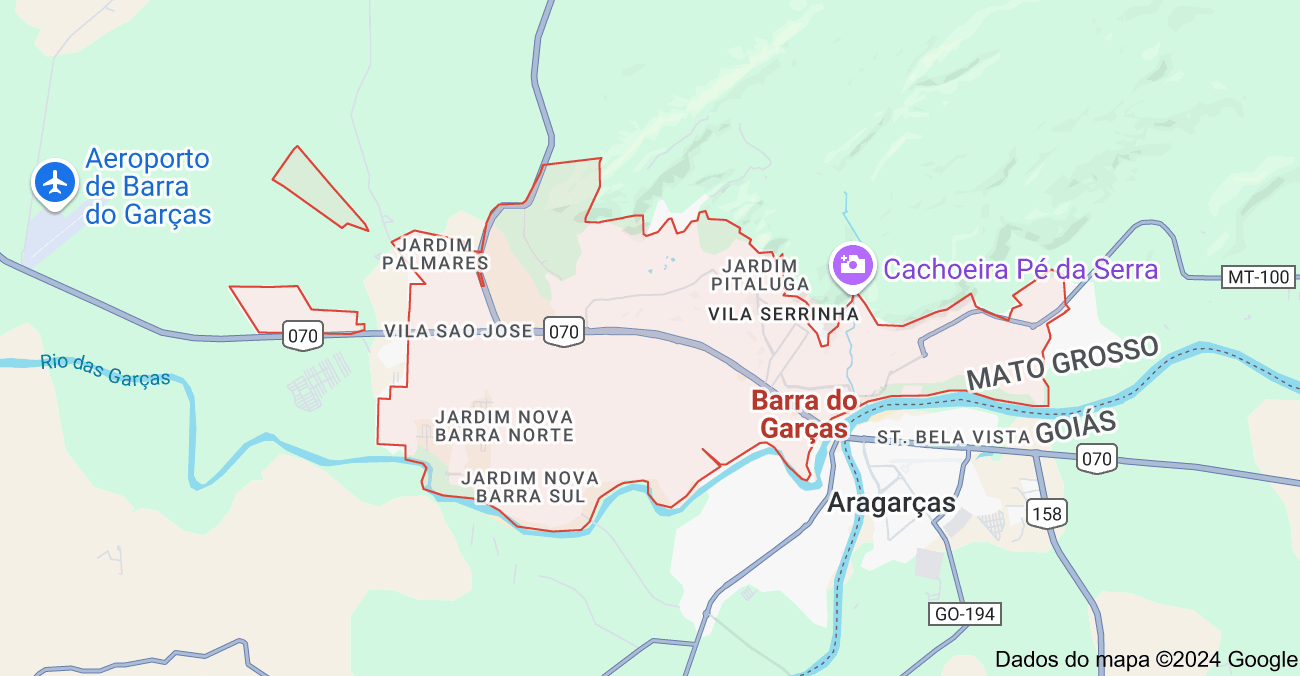
\includegraphics[width=0.5\linewidth]{barradasgarças.png}
%     \caption{Mapa de Barra das Garças}
%     \label{fig:mapa}
% \end{figure}

\section{Início}

Os agentes chegam de carro na cidade, às duas horas da tarde e com muita fome.
O carro não tem identificação, os agentes não podem usar de nenhum cargo oficial.

